\documentclass[conference]{IEEEtran}
\IEEEoverridecommandlockouts
% The preceding line is only needed to identify funding in the first footnote. If that is unneeded, please comment it out.
\usepackage{cite}
\usepackage{amsmath,amssymb,amsfonts}
\usepackage[super]{nth}
\usepackage{algorithmic}
\usepackage{graphicx}
\usepackage{textcomp}
\usepackage{xcolor}
\def\BibTeX{{\rm B\kern-.05em{\sc i\kern-.025em b}\kern-.08em
    T\kern-.1667em\lower.7ex\hbox{E}\kern-.125emX}}
\begin{document}

\title{VirNet: A deep neural network for viral sequence identification}


\author{
\IEEEauthorblockN{Aly O. Abdelkareem}
\IEEEauthorblockA{\textit{Department of Computer Engineering} \\
\textit{Ain Shams University}\\
Cairo, Egypt \\
aly.osama@eng.asu.edu.eg}
\and
\IEEEauthorblockN{Mahmoud I. Khalil}
\IEEEauthorblockA{\textit{Department of Computer Engineering} \\
\textit{Ain Shams University}\\
Cairo, Egypt \\
mahmoud.khalil@eng.asu.edu.eg}
\and
\IEEEauthorblockN{Hazem M. Abbas}
\IEEEauthorblockA{\textit{Department of Computer Engineering} \\
\textit{Ain Shams University}\\
Cairo, Egypt \\
hazem.abbas@eng.asu.edu.eg}
\and
\IEEEauthorblockN{Ali Elbehery}
\IEEEauthorblockA{\textit{Institute of Virology} \\
	\textit{HelmholtzZentrum München}\\
	München, Germany \\
	alielbehery@hotmail.com}
}

\maketitle

\begin{abstract}\\Metagenomics shows a promising understanding of function and diversity of the microbial communities due to the difficulty of studying microorganism with a pure culture isolation. Moreover, the viral identification is considered one of the most important steps in studying microbial communities. Several studies show different methods to identify viruses in mixed metagenomic data and phages in host genomes using homology and statistical techniques. These techniques have many limitations due to viral genome diversity. In this work, we propose a sequence deep model for viral identification of metagenomic data.\\
\textbf{Results:} To test this method, we generate fragments of viruses and bacteria from RefSeq genomes with different lengths to find the best hyperparameters of our model. Then, We simulated both microbiome and virome high throughput data from our test-set genomes in order to validate our method. Finally, we applied our tool on a case study of two types of metagenomic data such as Roche 454 and Illumina. We found our sequence model reached 85.12\% of accuracy whereas VirFinder tool obtained 75.61\% with the same training and testing data.\\
\textbf{Conclusion:} We developed the first deep sequence network based on viral identification in large data. This tool will help us in expanding our knowledge in natural viral communities.
\end{abstract}

\begin{IEEEkeywords}
 Metagenomics, Deep Learning, Viruses, LSTM, Classification 
\end{IEEEkeywords}


\section{Introduction}

Metagenomics is the cultivation-independent analysis of the genetic information of the collective genomes of the microbes within a given environment based on its sampling \cite{izard2014metagenomics}. There is a small fraction of extant microbial life has been identified because of the difficulty to study microbiology with a pure culture isolation. Scientist reported that there are less than 5\% of microorganisms can be easily cultured(Need a reference). Metagenomic analysis process demonstrates a promising understanding of different microorganisms. It answers some questions about microorganisms in the collection such as Who is there?, What can they do? and what can they potentially do?.

Microorganisms are found everywhere on earth and they are very important in our life. They are essential to our life. In this study, our interest is in Prokaryotic Microorganisms
(e.g. Bacteria and Archaea) and viruses. Bacteria are unicellular and microscopic organisms that reproduce by binary fission. On the other hand, viruses are typically submicroscopic consists of genetic materials either(DNA or RNA) surrounded by a protective coat of proteins and can only replicate inside living host cells. 

Viruses have an impact on different microbial communities and virus-host interaction can change many ecosystems such as human health and aquatic life. Phages are viruses that mainly infect bacteria and archaea. Furthermore, phages are abundant in Microbiome. Scientists are using isolation and culture-independent techniques to study viral diversity and viral-host interactions in microbial communities. Those techniques have many limitations because of there is no universal marker gene for viruses. Some reported most of the sequenced viruses in NCBI RefSeq are from 5\% of known phyla of prokaryotic hosts \cite{roux2015viral}.

High throughput sequencing technology is used for metagenomic studies which can generate massive amounts of short read sequences from prokaryotic cells in microbial communities regardless of cultivability of the cells, and viruses are inevitably captured at the same time in these samples. Sequencing microbial samples found viral sequences along with prokaryotic hosts. A study found 4-17\% virus sequences in human gut prokaryotic metagenomes \cite{minot2011human}. Moreover, Cellular contamination is quite frequent even with a careful purification of viral particles and this is one of the main reasons why we need a tool that can differentiate between bacterial and viral sequences.

The classical approach to know who is in metagenomic data is to assemble the high throughput reads to contigs then search against know genomic database in order to know these microorganisms. This approach is very limited because it only finds viruses closely related to those we already know about. It is estimated that only about 15\% of viruses in the human gut microbiome and 10\% in the ocean have similarity to the known viruses \cite{ren2017virfinder}. 

Machine learning approaches have been used to classify and cluster data based on hand-made features. The deep neural network is one of machine learning methods that are considered as a state of the art category for general classification problems. Deep learning shows significant improvements in several artificial intelligence tasks for example image classification, speech recognition, and natural language processing. Moreover, It shows promising results with genomic data \cite{angermueller2016deep}. \\

In this paper, we introduce a deep sequence model, VirNet, to identify viral sequences from a mixture of virus and bacterial sequences and purify viral metagenomic data from bacterial contamination as well. This will lead to discover more new viruses and help us to understand their functionality and diversity in the ecosystem.

\section{Related Work}

There has been extensive prior work on viral identification. Recent work has focused on identifying phages in bacterial genomes. Several methods have used similarity search with the known genomes in order to find viral contigs. There are three types of recent tools:
\begin{enumerate}
	\item Phages from prokaryotic genomes
	\item Viral sequences in mixed metagenomic datasets
	\item Phages and Viral sequences. 
\end{enumerate} 

There are many methods to find phages from prokaryotic genomes such as Phage\_Finder \cite{fouts2006phage_finder}, Prophinder \cite{lima2008prophinder}, PHAST\cite{zhou2011phast}, and PhiSpy \cite{akhter2012phispy}. These tools are using similarity search to known viruses databases using features such as genes. Some of them such as PhiSpy integrates other features such as protein length, AT and GC skew, transcription strand direction and unique virus k-mers. They have many limitations as they failed to detect viral sequences in metagenomic data as the databases are outdated, limited and don't represent viral diversity in the environment. Moreover, It is not optimized to process a large number of contigs \cite{roux2015virsorter} as they depend on alignment and homology processing limitations. 

The second type is able to detect viral sequences in mixed metagenomic datasets such as VIROME \cite{wommack2012virome} and MetaVir\cite{roux2011metavir}. They are using similarity search with the databases as same as the first type and Also, they are searching against proteins. Some people are using DIAMOND \cite{buchfink2014Diamond} or Centrifuge \cite{kim2016centrifuge} as they are fast and efficient for microbial classification. The limitation of this approach is related to limited databases as they only search for known genomes. 

The third type is able to detect phages and viral sequences such as VirSorter \cite{roux2015virsorter}. VirSorter is using similarity search to viral databases and integrates other features such as viral hallmark gene, enrichment of viral-like genes, enrichment of uncharacterized genes which make it more accurate but it has many limitations such as it require at least 3 genes within the contig as the smallest virus genome contains 3 genes so it has the same limitations as previous techniques because of using homology strategy. Moreover, it cannot work with short fragments or contigs and it is very slow in processing metagenomic datasets. 

Recently VirFinder \cite{ren2017virfinder} applied machine learning techniques. VirFinder is a statistical method based on the logistic regression model. It uses the K-mer feature which is considered as a discrimination feature for different sequence problems. It shows a great success with short sequences too and They found a great k-mer similarity score with viruses within other prokaryotic genomes. 

% need to write deep learning techniques in fragments classification

In this paper, we are using deep learning techniques which is much more suitable to sequence problems and also shows significant improvements to other machine learning models. In deep neural networks, the model will extract the most appropriate features during training which lead to better identification accuracy. 

\section{Materials and Methods}

We downloaded Viruses, Bacteria and Archaea genomes from RefSeq database then we split it into a train, valid and test genomes. Then, We took random non-overlapping fragments of different lengths (n= 100,150,300,500,1000). We divided the data into viral and non-viral with an approximate number to make the data balanced as the DNN models don't learn well from unbalanced data. Figure \ref{fig:data_pipline} shows the data pipeline. Table \ref{table:genome_stats} is the number of genomes we used in training and testing. We downloaded all the viruses genomes until Nov. \nth{1}, 2017 but we sampled bacterial genomes.

\begin{figure}
	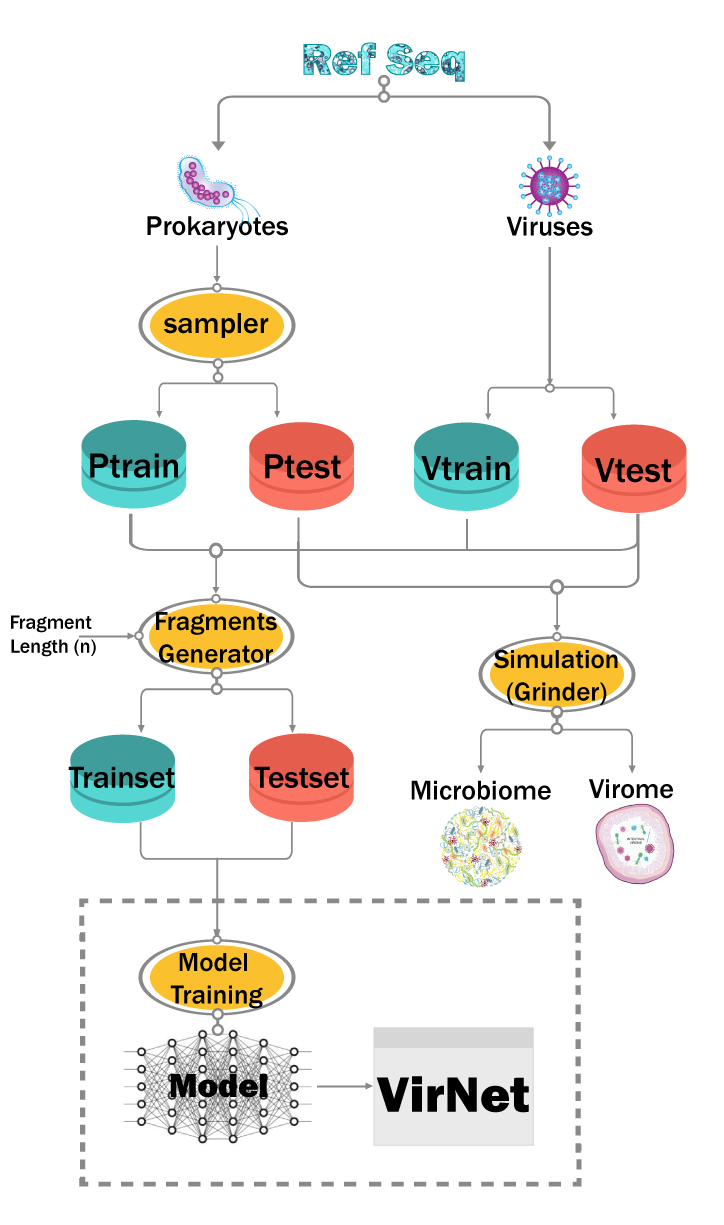
\includegraphics[width=\linewidth]{imgs/data_pipeline.PNG}
	\caption{VirNet Data Pipeline}
	\label{fig:data_pipline}
\end{figure}

\begin{table}[h!]
	\centering
	\begin{tabular}{||c c c||} 
		& Viruses & Bacteria \& Archaea \\ [0.5ex] 
		\hline\hline
		Total & 9556  & 178784  \\ 
		Train & 7686  & 143241  \\
		Test & 1870  & 35543  \\ [1ex] 
	\end{tabular}
	\caption{RefSeq Genomes}
	\label{table:genome_stats}
\end{table}

Moreover, We generated two metagenomic data Virome and Microbiome of 1M reads (100bp) using Grinder \cite{angly2012grinder} with our test genomes to simulate shotgun metagenomic sequences. Additionally, We used Illumina error model indicated by mutation\_dist poly4 3e-3 3.3e-8 and mutation ratio 91:9 (9 indels for each 91 substitution mutations) because for Illumina indel errors occur more often than substitution errors \cite{laehnemann2015denoising}. Table \ref{table:simulate_stats} shows simulated data statistics.  \\

\begin{table}[h!]
	\centering
	\begin{tabular}{||c c c||} 
		& Microbiome & Virome \\ [0.5ex] 
		\hline\hline
		Bacteria Length & 75450367  bp  & 17551396 bp  \\
		Bacteria Genomes & 1488 & 422\\
		Bacterial reads & 803742 & 176059\\
		Viruses Length & 25133078 bp  & 52609236 bp  \\ 
		Viruses Genomes & 845 & 1870\\
		Viral reads & 196258 & 823941 \\  
		Viral Ratio & 25.00\% & 75.00\% \\ 
		Library coverage &  0.994x &  1.001x  \\
		Diversity (richness) & 2302 & 2726 \\ [1ex]
	\end{tabular}
	\caption{Grinder Simulated Metagenome}
	\label{table:simulate_stats}
\end{table}

The deep neural network could learn how to extract suitable features from the raw data. Recurrent neural networks (RNN), long short-term memory (LSTM) \cite{hochreiter1997long} and gated recurrent neural networks (GRU) \cite{chung2014empirical} can model complex sequences and have been used for sequence modeling problems. LSTM is an RNN network capable of learning long-term dependencies and solves the vanishing gradients during training. We trained a sequence model \ref{fig:model_diagram} its input is the DNA nucleotide bases with 100bp fragments. The output is a binary with a probability of this fragment if it is viral or non-viral. The model architecture consists of 2 stacked layer of LSTM with 128 neurons and a dense layer with 64 neurons to embedding the fragment vector for clustering or reduce its dimension. We added a 20\% as a dropout ratio to avoid over-fitting. 


\begin{figure}
	\centering
	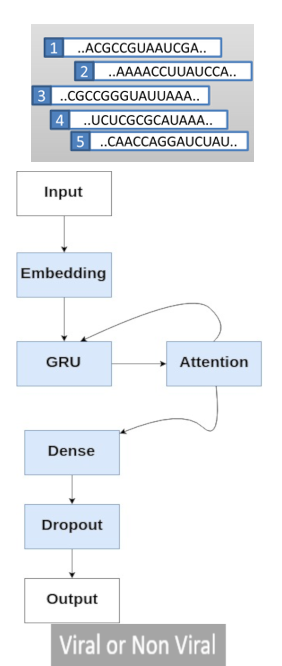
\includegraphics[width=0.5\columnwidth]{imgs/model_diagram.PNG}
	\caption{VirNet Model architecture}
	\label{fig:model_diagram}
\end{figure}

Then, we applied our tool to two real metagenomes as a case study
\begin{enumerate}
	\item \textbf{454}: Subtropical freshwater microbial and viral metagenome (SRR648314).\
	\item \textbf{Illumina}: Lake Michigan virome (SRX995836).
\end{enumerate}
Our tool is able to read not only fasta files and fastq files. Furthermore, it is able to deal with paired-end reads i.e. if one of the two pairs is identified as a virus, the other should be the same. If there are conflicts between the classifications of the two pairs; this pair could be denoted as ambiguous.


\section{Results}

To test this method, we generate fragments of viruses and bacteria from RefSeq genomes with different lengths to find the best hyperparameters of our model. Then, We simulated both microbiome and virome high throughput data from our test-set genomes in order to validate our method. Finally, we applied our tool on a case study of two types of metagenomic data such as Roche 454 and Illumina. We found our sequence model reached 85.12\% of accuracy whereas VirFinder tool obtained 75.61\% with the same training and testing data. Table \ref{table:model_results} shows experiment results.

\begin{table}[h!]
	\centering
	\begin{tabular}{||c c c||} 
		Model &	Accuracy&	ROC-AUC \\ [0.5ex] 
		\hline\hline
		LSTM ( 1L , 128 N ) + DNN ( 64 N ) &	79.80\% &	80\% \\
		LSTM ( 2L , 128 N ) + DNN ( 64 N ) &	82.88\%	& 83\% \\
		LSTM ( 3L , 128 N )  &	80.32\%	& 81\% \\ 
		LSTM ( 2L, 64 N ) &	79.20\%	& 79.50\% \\ 
		LSTM ( 2L, 256 N ) &	78.70\%	& 79\% \\
		RNN ( 2L ) &	81.30\%	& 81\% \\
		GRU ( 2L ) &	82.10\% &	82\% \\
		LSTM ( 2L, 128 N, 0.2 dropout) &	\textbf{85.12\%} 	& 85\% \\
		VirFinder ( Benchmark ) &	\textbf{74.40\%} &	74\% \\[1ex]
	\end{tabular}
	\caption{Hyperparamters optimization results}
	\label{table:model_results}
\end{table}

We tried different fragment length (n=100,500,1000,3000) with VirFinder and we found that VirFinder cannot identify viruses 100 bp. See figure \ref{fig:roc_auc_virfinder} and table \ref{table:virfinder_results}.

\begin{figure}
	\centering
	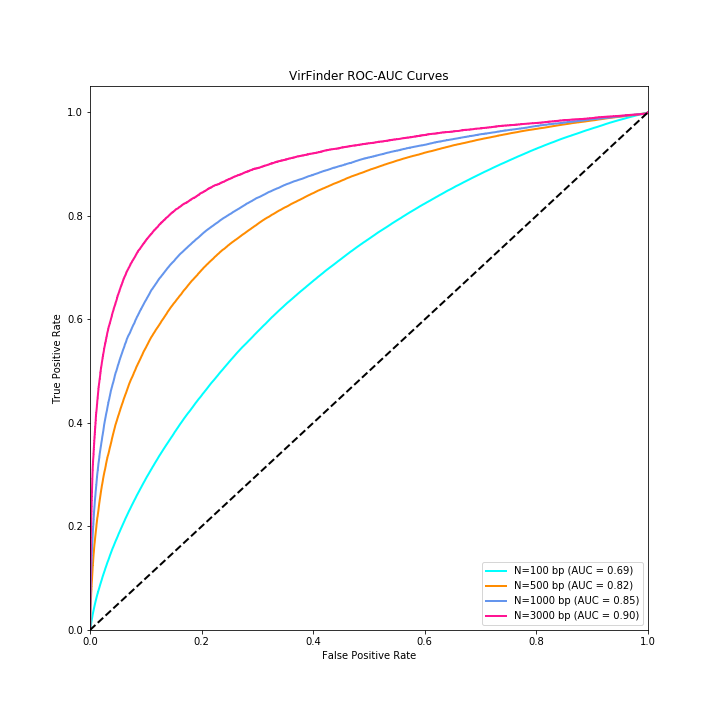
\includegraphics[width=\columnwidth]{imgs/roc_auc.png}
	\caption{VirFinder ROC-AUC curves}
	\label{fig:roc_auc_virfinder}
\end{figure}


\begin{table}[h!]
	\centering
	\begin{tabular}{||c c c c c||} 
		Length(N) &	Accuracy & Avg. Precision & Avg. Recall &	ROC-AUC Score \\ [0.5ex] 
		\hline\hline
		100 &	63.9\%	& 0.64 & 0.64 & 0.64 \\
		500 &	75.61\% &	0.76 & 0.76 & 0.75 \\
		1000 &	80.28\% & 0.82 & 0.80 & 0.78 \\
		3000 &	87.11\% & 0.88 & 0.87 & 0.83\\[1ex]
	\end{tabular}
	\caption{VirFinder Results on our test-set}
	\label{table:virfinder_results}
\end{table}


We tried VirFinder on the simulated metagenomes and we found that VirFinder accuracy is arround 65\%. See figure \ref{fig:roc_auc_virfinder_simulated} and table \ref{table:virfinder_results_simulated}.

\begin{figure}
	\centering
	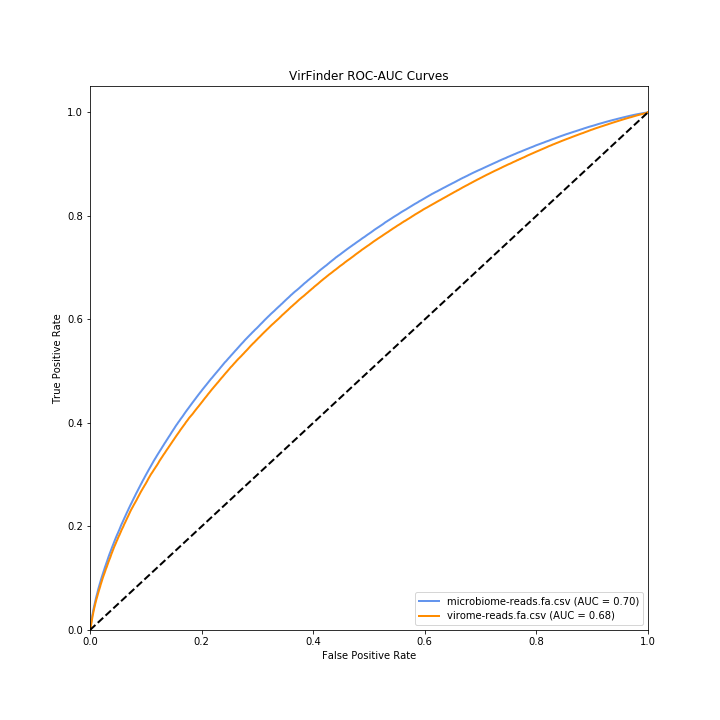
\includegraphics[width=\columnwidth]{imgs/roc_auc_simulated.png}
	\caption{VirFinder ROC-AUC curves on Simulated metagenomes}
	\label{fig:roc_auc_virfinder_simulated}
\end{figure}



\begin{table}[h!]
	\centering
	\begin{tabular}{||c c c c c||} 
		Length(N) &	Accuracy & Avg. Precision & Avg. Recall &	ROC-AUC Score \\ [0.5ex] 
		\hline\hline
		Virome &	62.77\%	& 0.72 & 0.63 & 0.63 \\
		Microbiome &	64.49\% &	0.72 & 0.64 & 0.64 \\ [1ex]
	\end{tabular}
	\caption{VirFinder Results on our Simulated Metagenomes}
	\label{table:virfinder_results_simulated}
\end{table}

\section{Discussion}

In our tool, there are no handmade features as the network will learn how to extract appropriate features for the raw data. It shows better accuracy as it is trained with the updated viral databases with a good statistical model. This helps us to generalize this model with all genomes and to make a generalized model for sequence classification. We also able to identify the short viral sequences as LSTM learns from the dependences between the input sequence. 
There is no evidence that these training prokaryotic genomes don't have viral infection or not. We need clean the training genomes to get better accuracy. Additionally, Using GPUs in this tool make it very fast and scalable with a large number of sequences. We found VirNet 16X faster than normal methods. 

\section{Conclusion}

We developed the first deep sequence network based on viral identification in large data. This tool will help us in expanding our knowledge in natural viral communities.

\section*{Acknowledgments}

We would like to thank everyone for their help and supervision.


\bibliography{scholar}
\bibliographystyle{plain}


\end{document}
